\chapter{Le modèle physique} \label{ch:introduction_physique}


\section{observation -> Hubble}

découverte des galaxies\\
découverte de l'expansion de l'univers


\begin{figure}[bth]
        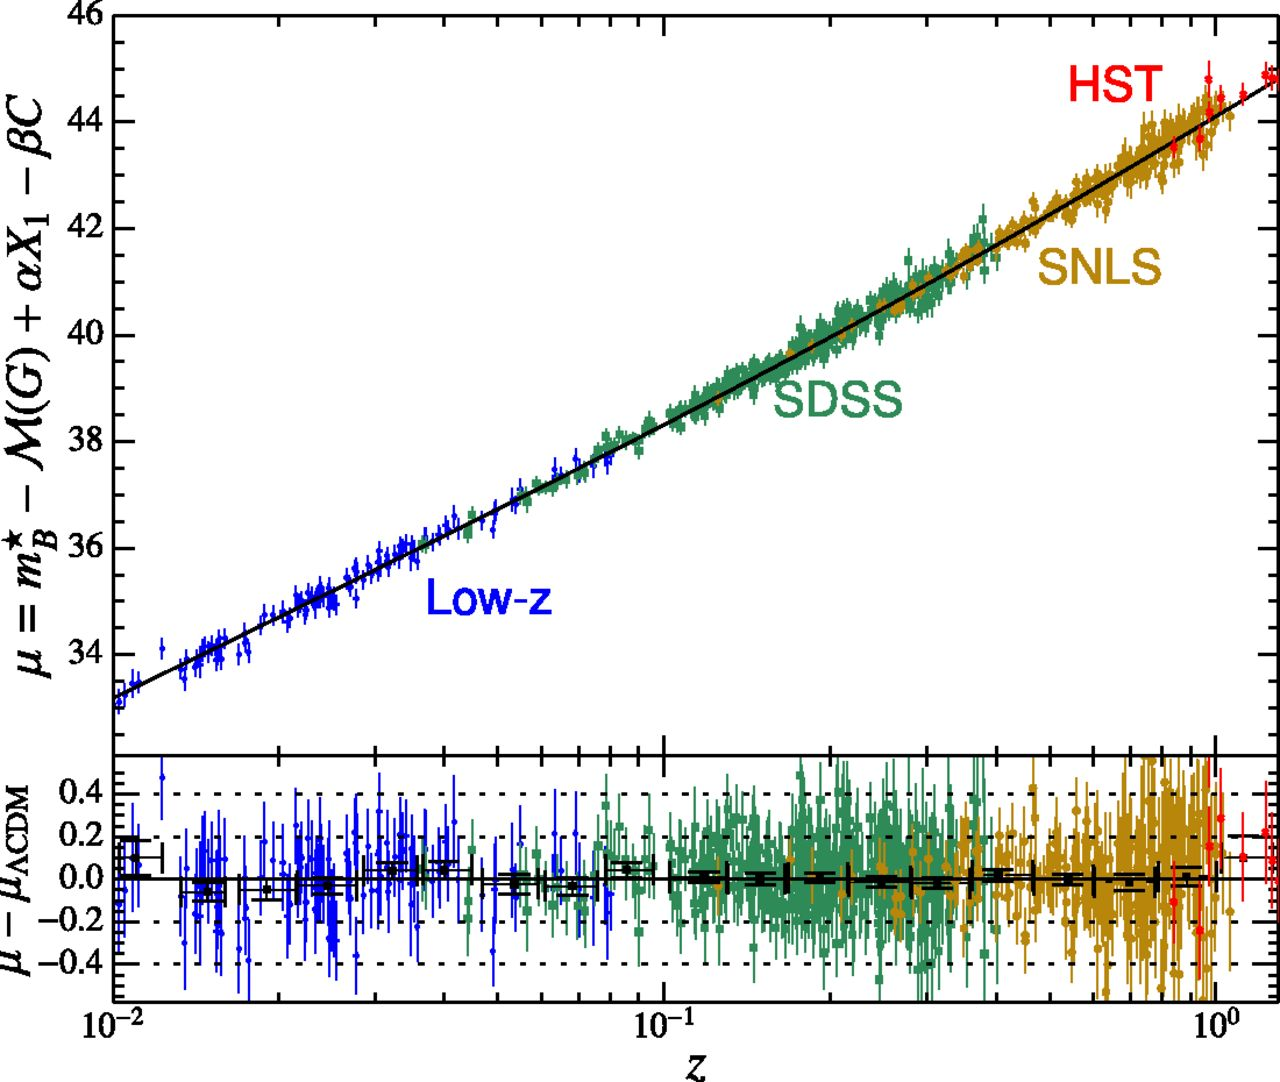
\includegraphics[width=.9\linewidth]{img/01/hubble_law.jpg} 
        \caption{Hubble law. 
%http://www.pnas.org/content/112/11/3173/F2.expansion.html
        Image ESO}
 		\label{fig:hubble_law}
\end{figure}

\begin{equation}
V = H_0 D
\end{equation}


\begin{figure}[bth]
        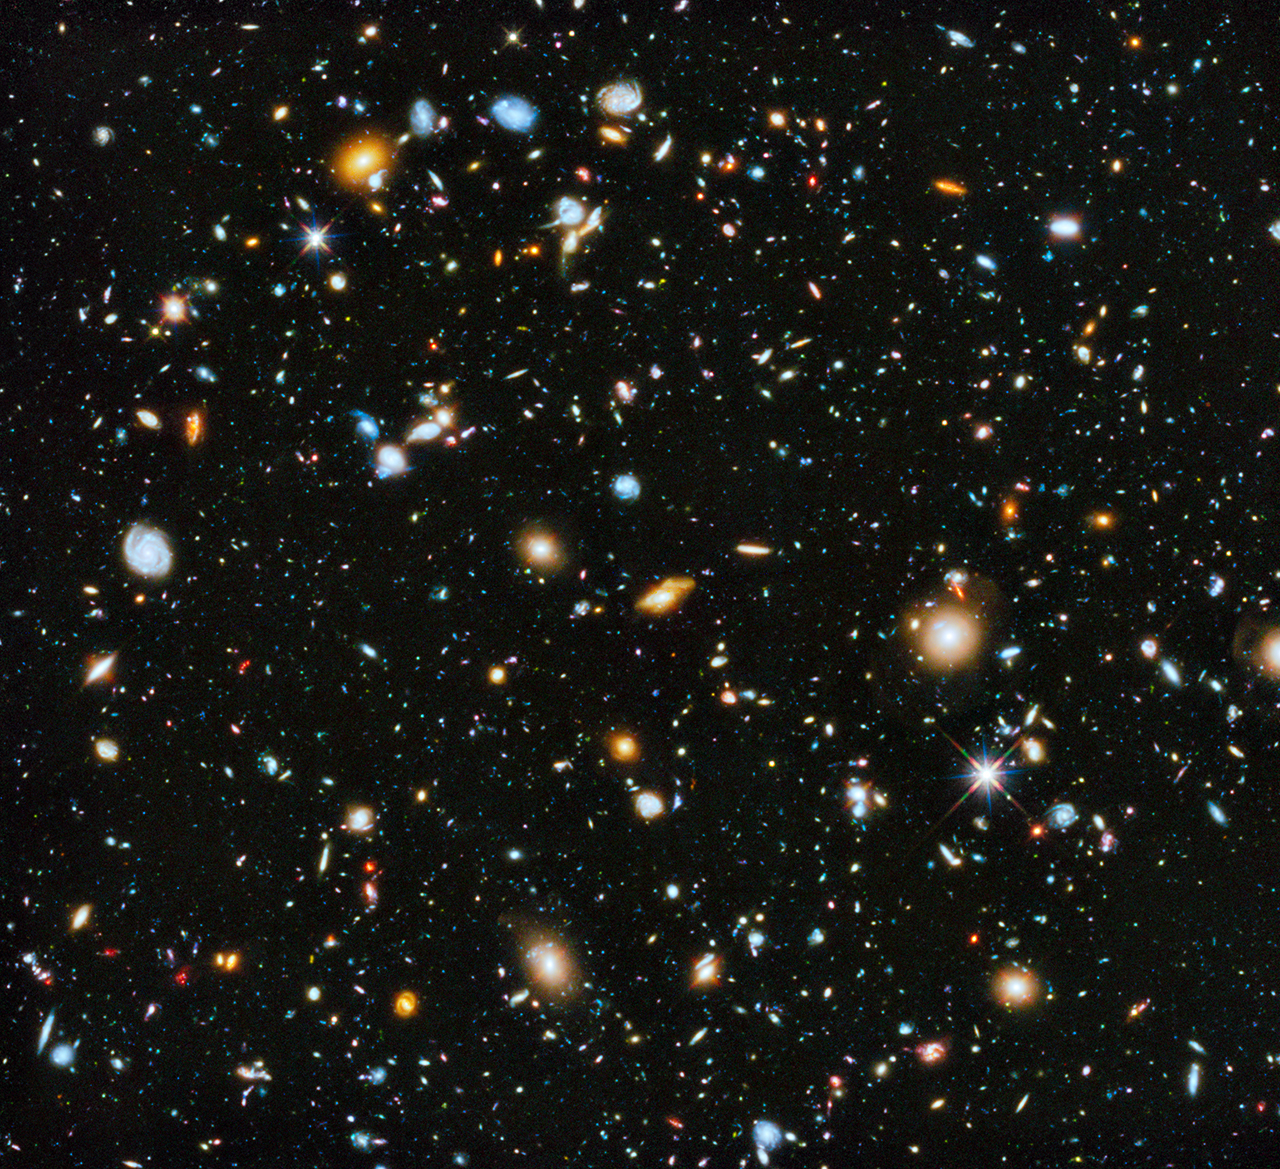
\includegraphics[width=.9\linewidth]{img/01/hudf.jpeg} 
        \caption{Hubble Ultra Deep Field 2014. 
        Image NASA}
 		\label{fig:hubbl_deep_field}
\end{figure}

\section{théorie - lCDM}

le big bang\\
l'inflation\\
la nucléosynthèse\\
le CMB\\
la reionization


\section{Le CMB}


\subsection{Observations}

Penzias et Willson

\subsection{Théorie}

surface de dernière diffusion


\subsection{Température}
Le cosmic Microwawe background se presente sous la forme du corp noir le plus parfait connus.
Fig. \ref{fig:cmb_thermal_spectrum}
T=2.73K


\begin{figure}[bth]
        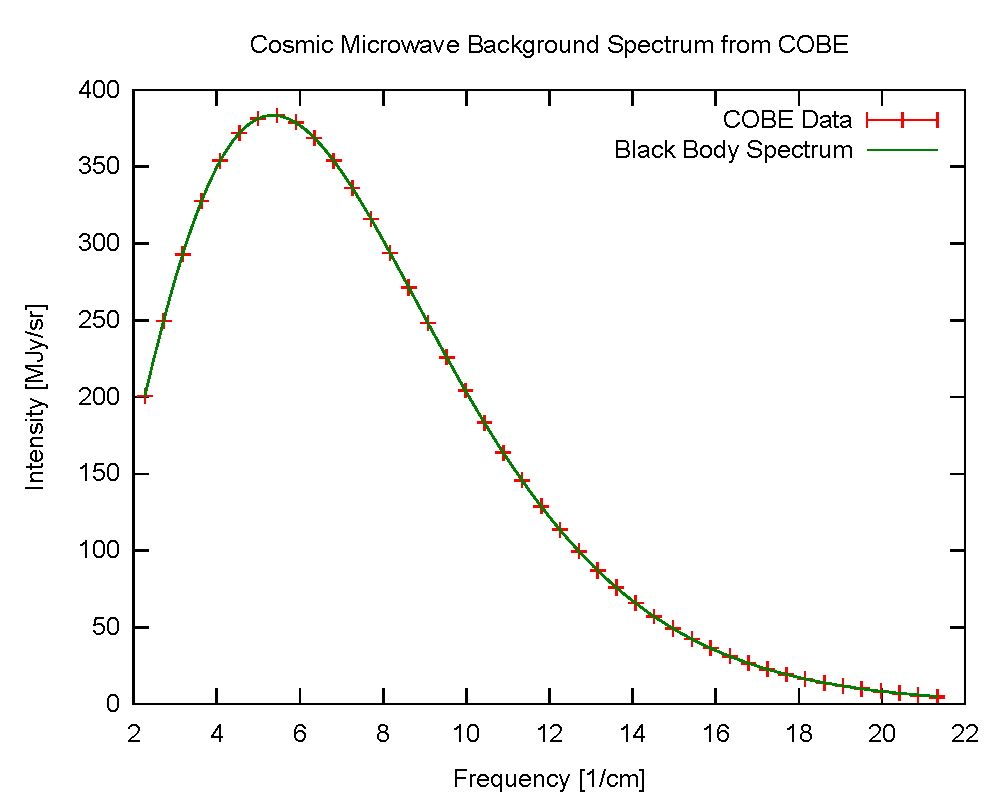
\includegraphics[width=.95\linewidth]{img/01/Cmbr.pdf} 
        \caption{Spectre thermique du CMB vue par le satellite Cosmic Background Explorer (COBE). 
        Image Wikipédia}
 		\label{fig:cmb_thermal_spectrum}
\end{figure}




\subsection{Spectre de puissance}

Le CMB n'est pas uniforme, il presente de tres faibles fluctuations (1e-5)qui nous renseigne sur l'etat de l'univers au moment de son emission.
Fig. \ref{fig:cmb_power_spectrum}

\begin{figure}[bth]
        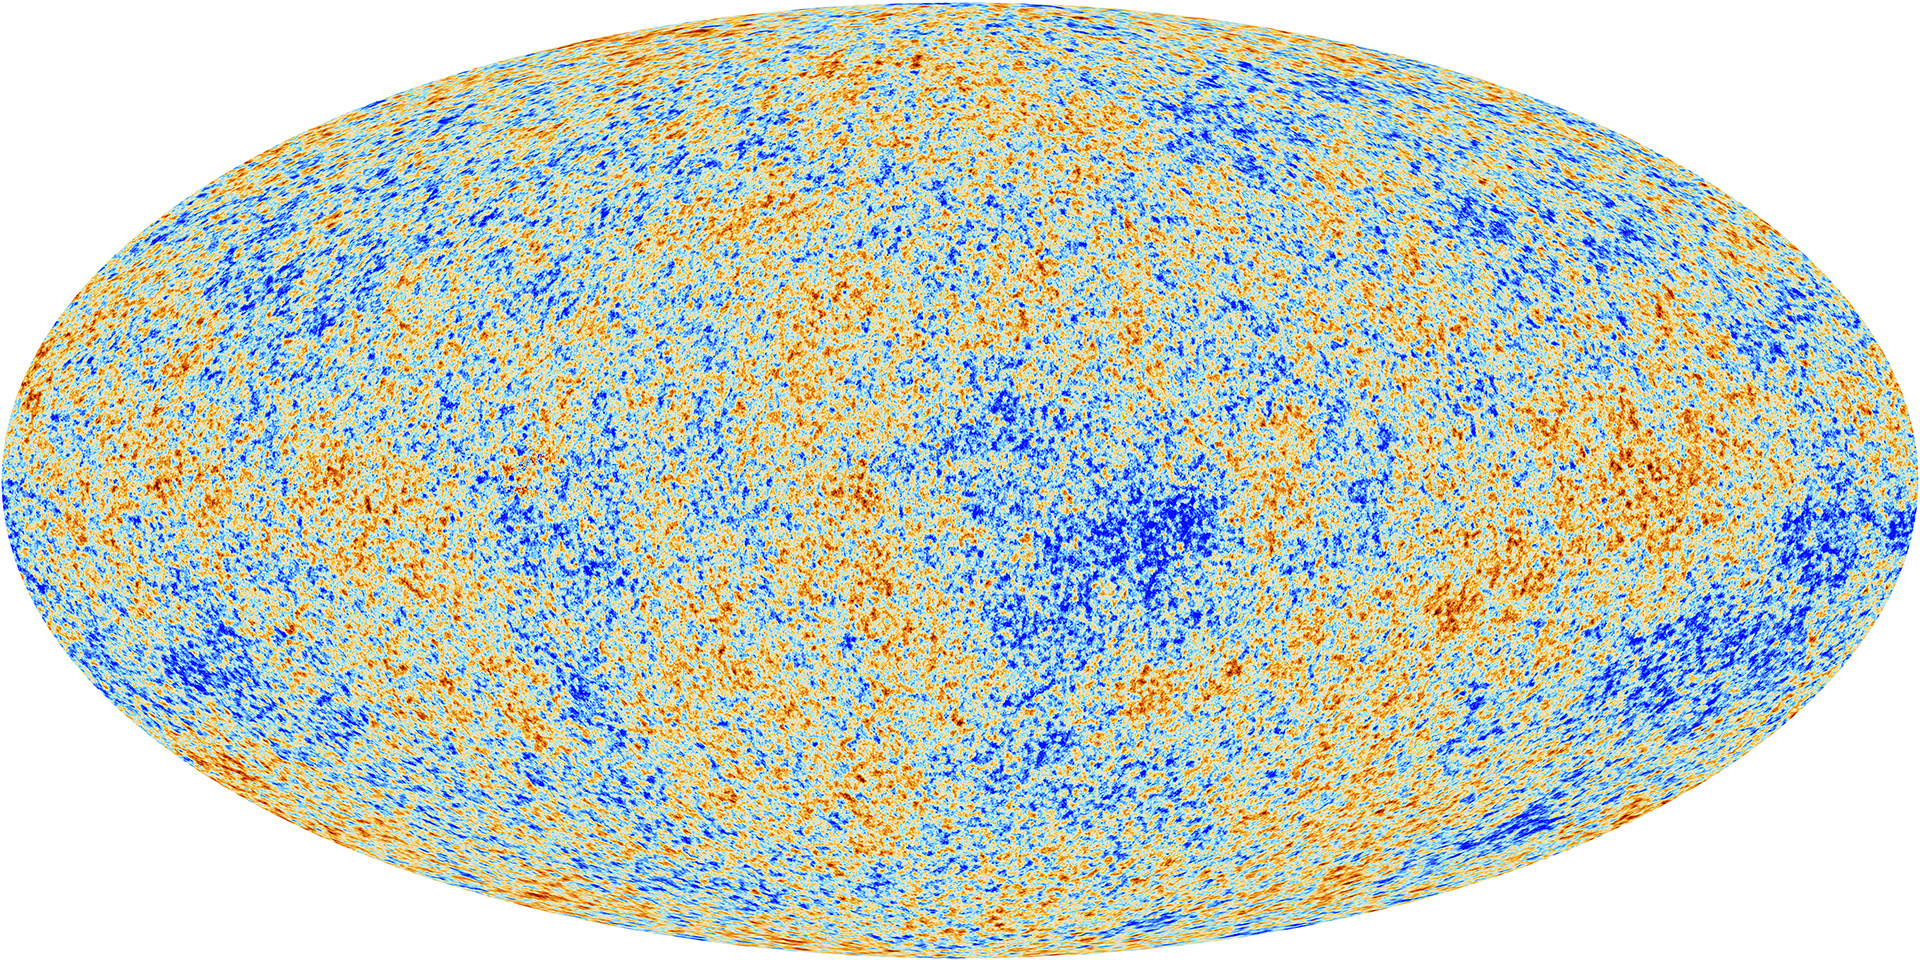
\includegraphics[width=.95\linewidth]{img/01/CMB.jpeg} 
        \caption{Les fluctuation du CMB vues par le satellite Planck. 
        Image ESA}
 		\label{fig:cmb}
\end{figure}


En decomposant ces fluctuations en harmoniques sphériques:
Fig\,\ref{fig:harmoniques_spheriques}

decomposition en multipoles
%https://www.physicsforums.com/threads/can-someone-explain-angular-power-spectrum.309483/
\begin{equation}
 \frac{\Delta T(\theta,\phi)}{T} = \sum_{l>0} \sum_{m=-l}^l a_{lm} Y(\theta,\phi)_{lm}
\end{equation}

avec : 

\begin{equation}
a_{lm}= \int d\Omega(\theta,\phi) \Delta T (\theta,\phi) Y(\theta,\phi)_{lm}
\end{equation}

\begin{figure}[bth]
        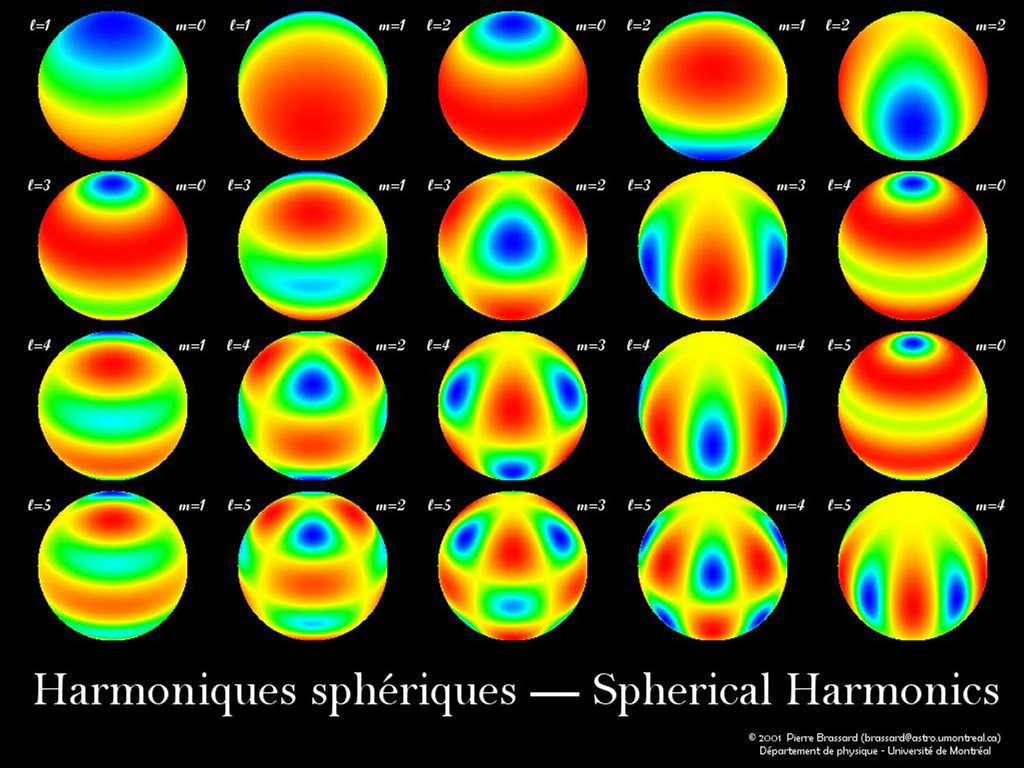
\includegraphics[width=.95\linewidth]{img/01/harmoniques_spheriques.jpeg} 
        \caption{
        représentation des $Y(\theta,\phi)_{lm}$
 Pierre Brassard, université de Montréal 
%Spectre thermique du CMB vue par le satellite Cosmic Background Explorer (COBE). 
        Image Wikipédia}
 		\label{fig:harmoniques_spheriques}
\end{figure}


\begin{equation}
C_l = \frac{1}{2l+1} \sum_{m=-l}^l a_{lm} a_{lm}^*
\end{equation}


Et finalement, on obtient le spectre de puissance:

\begin{equation}
D_l = \frac{l (l+1) C_l }{2 \pi} 
\end{equation}

représenté Fig.\,\ref{fig:cmb_power_spectrum}

\begin{figure}[bth]
        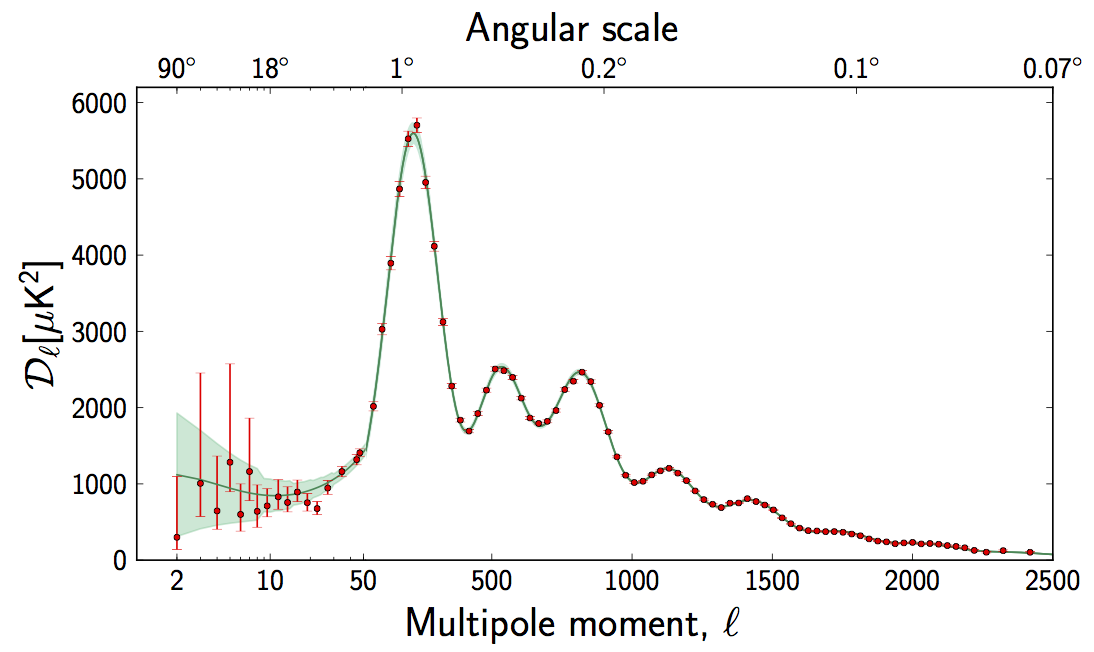
\includegraphics[width=.95\linewidth]{img/01/CMB_power_spectrum.png} 
        \caption{Spectre de puissance des fluctuation du CMB.
        Image ESA}
 		\label{fig:cmb_power_spectrum}
\end{figure}


\section{Le contenu de l'univers - (Théorie)}

Pour simuler l'univers, on a besoin de savoir ce qu'il contient. 
A partir du spectre de puissance, on peut déterminer les différentes composantes de l'univers (paramètres cosmologique).

univers infini, homogène, isotrope


%https://ned.ipac.caltech.edu/level5/Freedman2/Freed6.html


\begin{figure}[bth]
        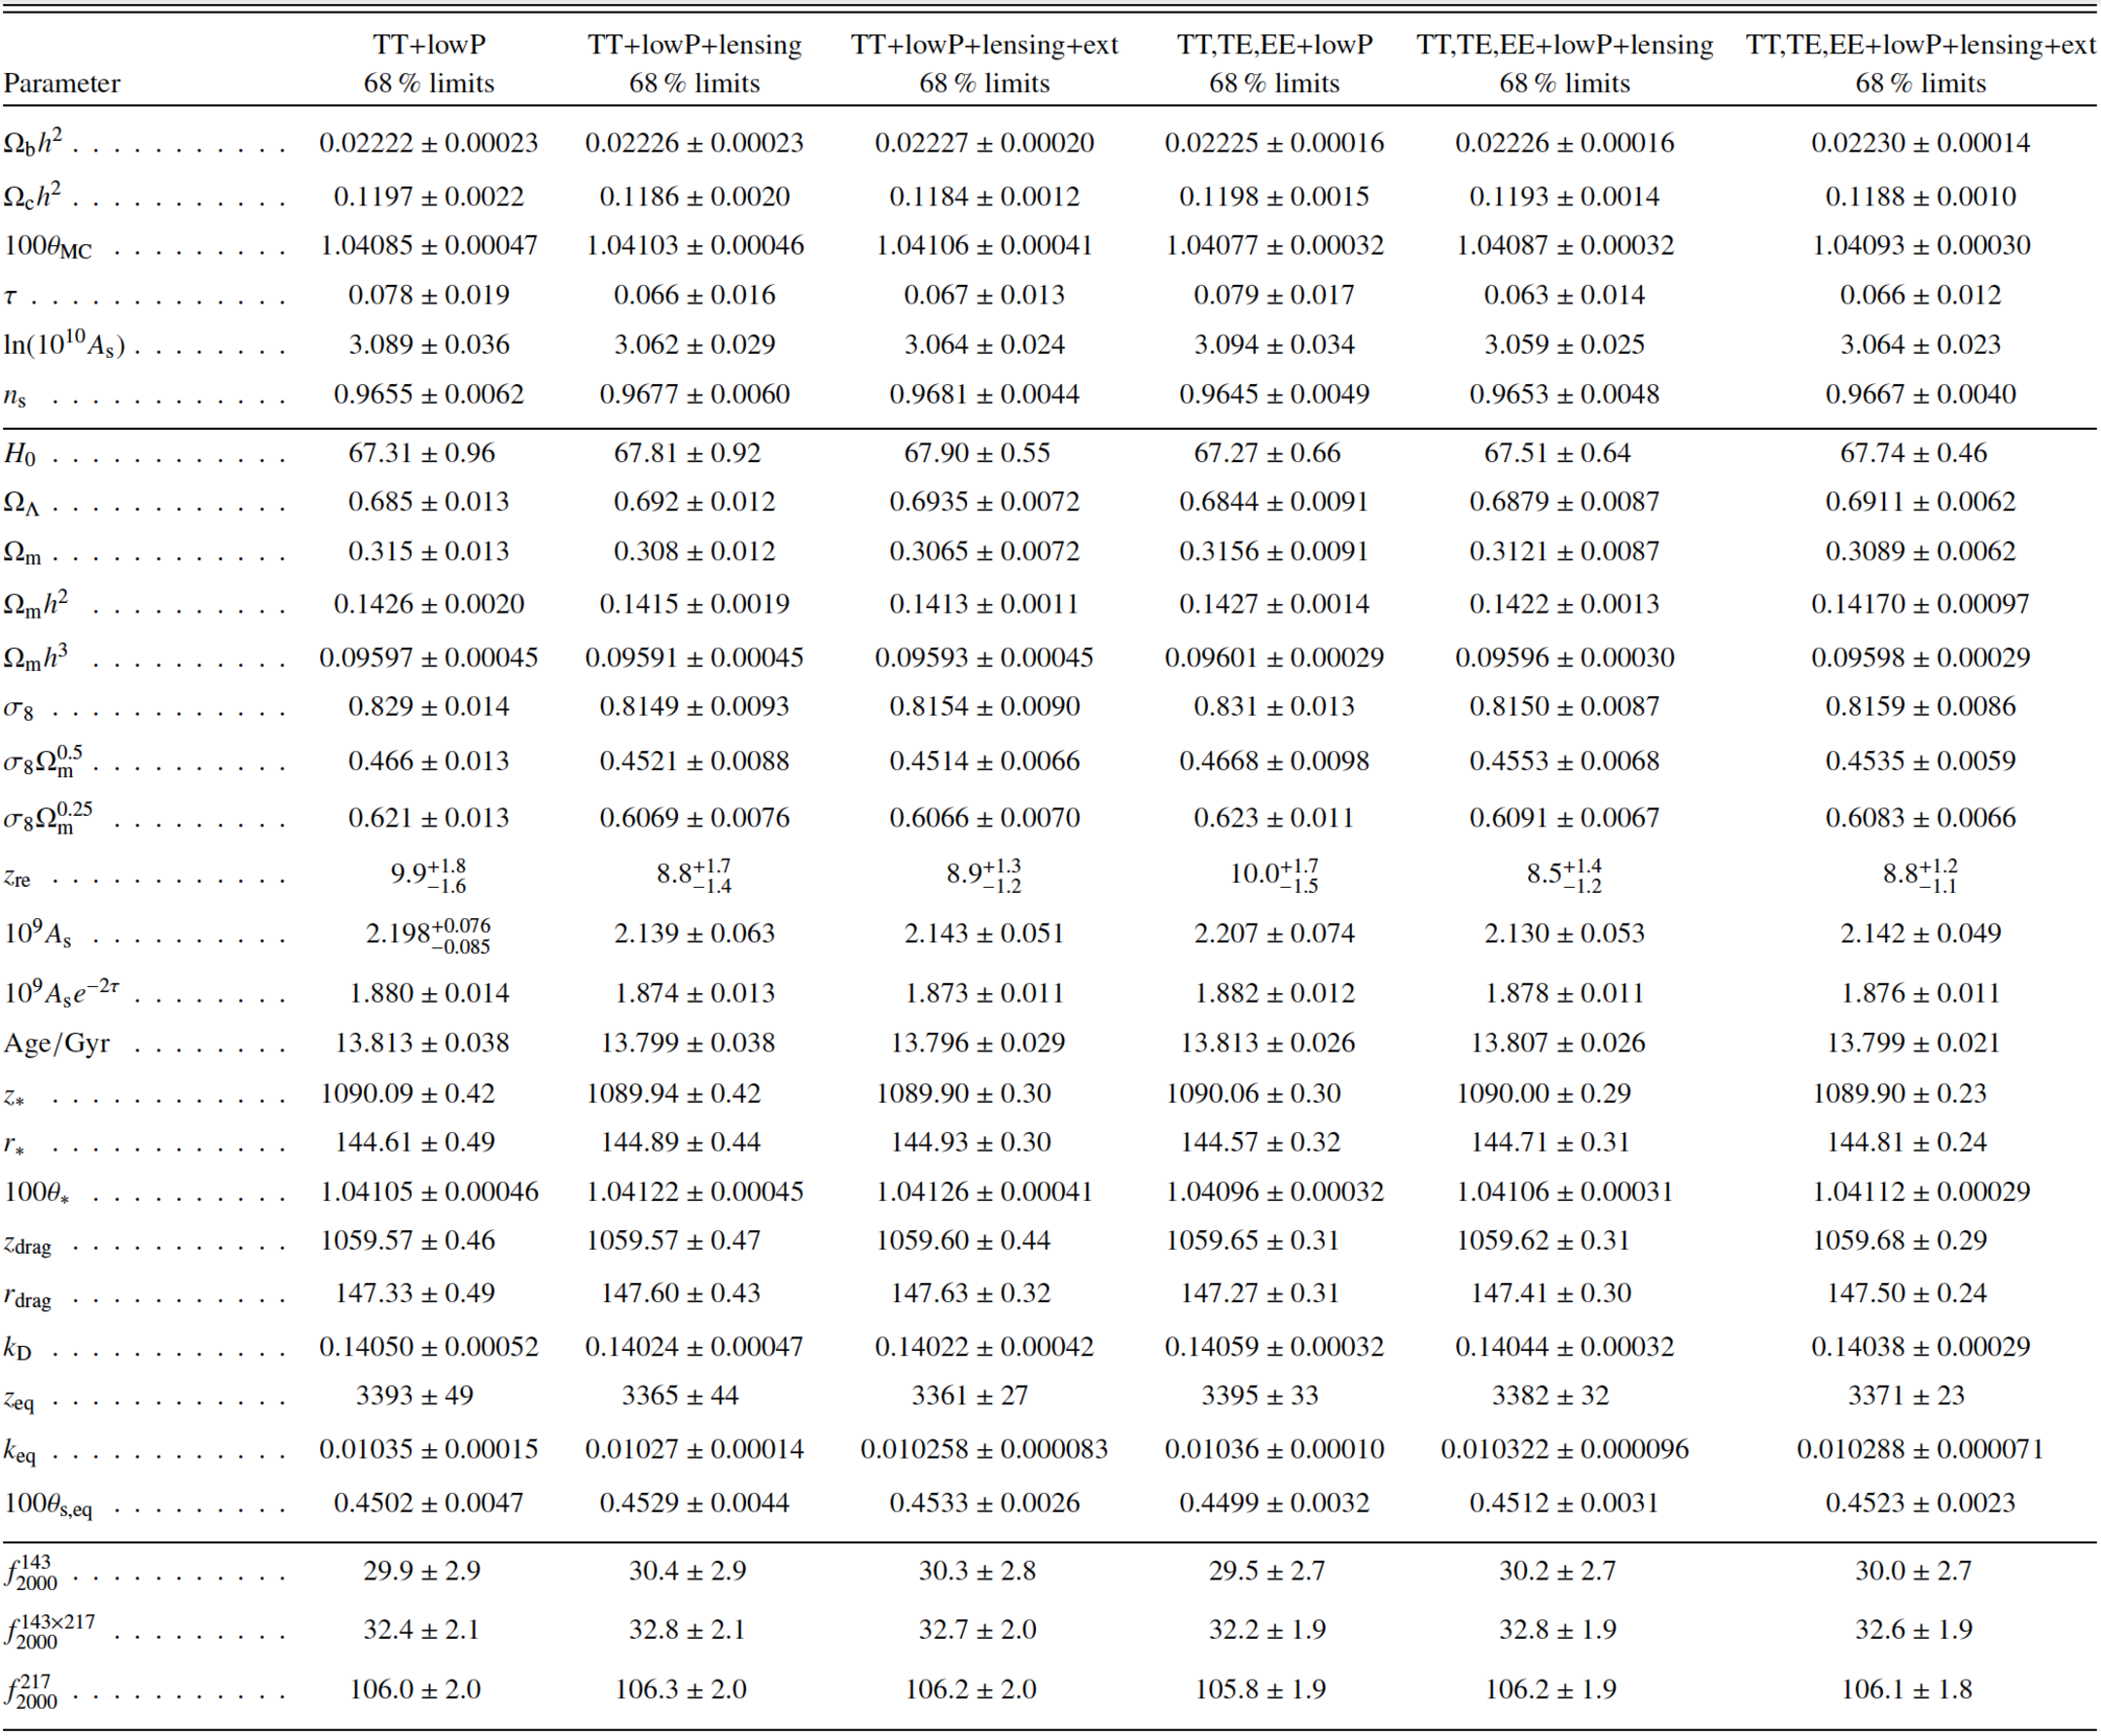
\includegraphics[width=.95\linewidth]{img/01/table_planck.pdf} 
        \caption{Determination des parametres cosmologiques par la colaboration Planck.}
 		\label{fig:planck_parameters}
\end{figure}

\citep{planck_collaboration_planck_2016}

\subsection{Energie noire $\Lambda$}

\subsubsection{Equation d'Einstein}

La notion d'un univers non statique a ete introduite par Einstein en 1917 en rapport avec ses travaux sur le relativité générale. 
Sa célèbre equation de champ décrivant le lien entre densité d'énergie et déformation de l'espace temps introduit la constante cosmologique $\Lambda$ representant 

Equation d'Einstein :
http://cdsads.u-strasbg.fr/abs/1915SPAW.......844E
\begin{equation}
R_{\mu\nu} = \frac{1}{2} g_{\mu\nu}R + \Lambda g_{\mu\nu}  = \kappa T_{\mu\nu}
\end{equation} 



Découverte de l'accélération de l'expansion de l'univers simultanément par 2 équipes :
Les 2 ont eue le prix nobel en 2011

\begin{itemize}
\item  Supernova Cosmology Project
 http://cdsads.u-strasbg.fr/abs/1999ApJ...517..565P
 
 \item  High-Z supernovae search team
http://cdsads.u-strasbg.fr/abs/1998AJ....116.1009R

\end{itemize}

quelques mois plus tard :
Première apparition du terme energie noire:
http://cdsads.u-strasbg.fr/abs/1999PhRvD..60h1301H



\subsubsection{ Équations de Friedmann }

 Recriture de l equation d'Einstein en considerant un univers homogene et isotrope.
 
 Alexandre Friedmann Über die Krümmung des Raumes, Zeitschrift für Physik 10, 377-386 (1922). Première écriture des équations de Friedmann, dans le cas d'une coubure spatiale positive. http://cdsads.u-strasbg.fr/abs/1922ZPhy...10..377F 
(de) Alexandre Friedmann, Über die Möglichkeit einer Welt mit konstanter negativer Krümmung des Raumes, Zeitschrift für Physik 21 326–332 (1924). Écriture des équations de Friedmann dans le cas d'une courbure spatiale négative. 
 
univers de Friedmann-Lemaître-Robertson-Walker  
http://dictionnaire.sensagent.leparisien.fr/%C3%89quations%20de%20Friedmann/fr-fr/
 
Équations de Friedmann : 
\begin{equation}
3 \left( \frac{H^2}{c^2} +\frac{K}{a^2} \right) = \frac{8 \pi G }{c^2} \rho
\label{eq:friedman1}
\end{equation}

\begin{equation}
-2 \frac{ \dot{H}}{c^2} -3 \frac{H^2}{c^2} -\frac{K}{a^2} = \frac{8 \pi G }{c^4 P}
\label{eq:friedman2}
\end{equation}

Eq. \ref{eq:friedman1} relie le taux d'expansion H, la courbure spatiale K et le facteur d'échelle a à la densité d'énergie $\rho$, 
Eq. \ref{eq:friedman2} relie la pression P à la dérivée temporelle du taux d'expansion
 
 
 
\begin{equation}
\frac{\dot{a}}{a} = H_0 \sqrt{ \Omega_{r,0} a^{-4} +  \Omega_{M,0} a^{-3} + \Omega_{K,0}a^{-2} + \Omega_{\lambda,0}  } 
\end{equation}


\begin{equation}
 \Omega_{i,0} = \frac{\rho_{i,0}}{\rho_{c,0}}
 \end{equation}

\begin{equation}
\rho_{c,0} = \frac{3H_0^2}{8\pi G}
 \end{equation}
 
 
\begin{equation}
 \Omega_{K,0} = 1 - \Omega_{r,0} - \Omega_{M,0} - \Omega_{\lambda,0} 
 \end{equation}

Univers plat
\begin{equation}
 \Omega_{K,0} = 0
 \end{equation}

\begin{equation}
\Omega_{\lambda,0} +  \Omega_{M,0} + \Omega_{r,0} =1
 \end{equation}




échelle gigaparsec\\
Facteur d'expansion


\begin{equation}
H=\frac{1}{a} \frac{da}{dt} = \frac{\dot{a}}{a}
\end{equation}

Metrique de Friedmann-Lemaître-Robertson-Walker (FLRW)

\subsection{Matière noire CDM}

echelle mega parsec
gouverne la gravité
non collisionnelle

\subsection{Baryon}

echelle kilo parsec
collisionnelle
interagit avec la radiation
La matière visible

\subsection{Radiation}

quasiment notre seul source d'information sur l'univers (plus vrai depuis les ondes gravitationnelles)
essentielle pour la reionization
seulement E>13.6 eV

\subsection{bilan}

plot en camembert avec les différents constituants

\section{Observation -> la reionization}

le manque d'observations

la difficulté des observations

les futures observations

Quelles sont les preuves de la réionisation?

\subsection{spectre de quasar}

tunnel gun peterson
\begin{figure}[bth]
        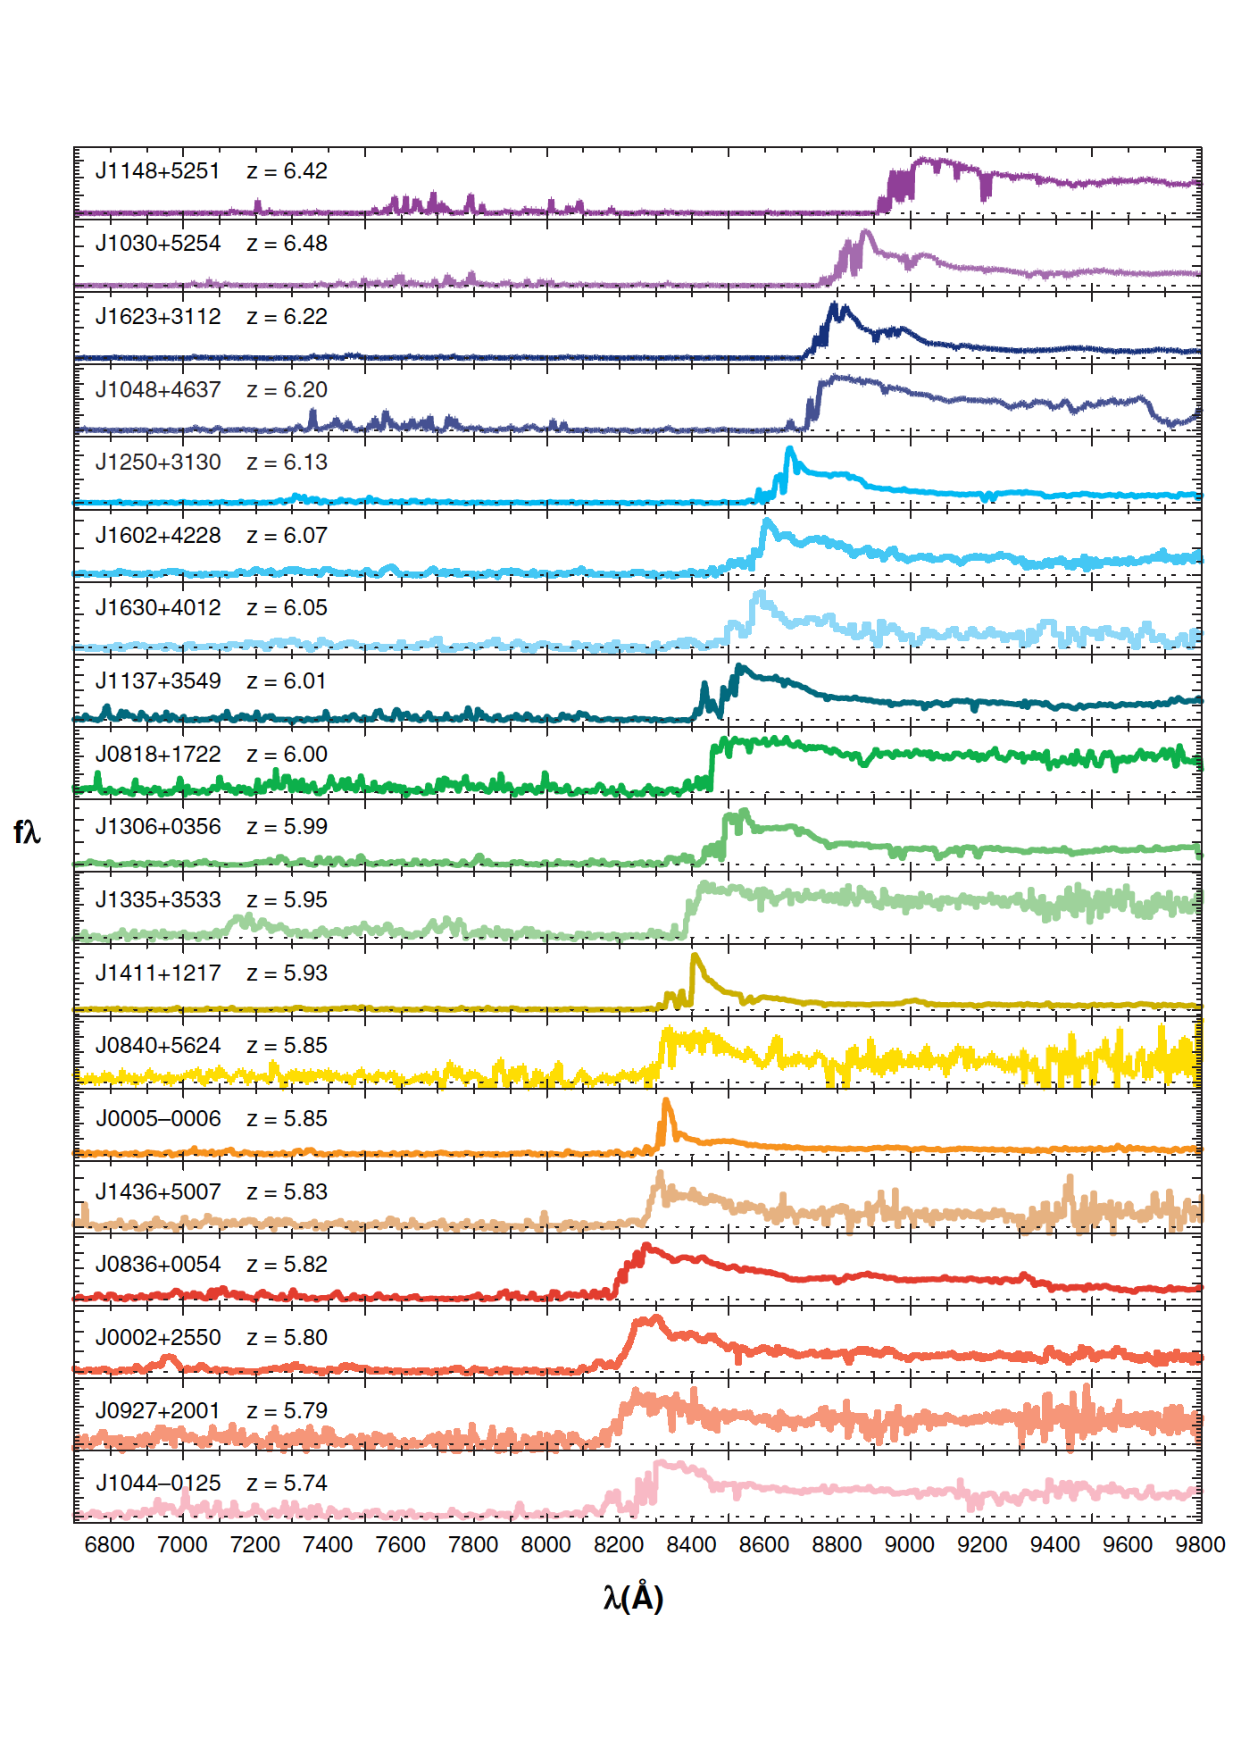
\includegraphics[width=.95\linewidth]{img/01/quasar_spectre.pdf} 
        \caption{Spectre de quasar a differents redshift presentant un tunnel gun peterson.
        Image fan et al.}
 		\label{fig:spectre_quasar}
\end{figure}

\subsection{Epaisseur optique lyman alpha}

\begin{figure}[bth]
        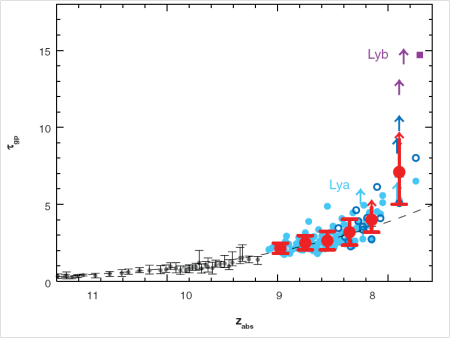
\includegraphics[width=.95\linewidth]{img/01/epaisseur_optique_quasar.png} 
        \caption{%https://ism2009.wordpress.com/2009/04/28/on-the-density-of-neutral-hydrogen-in-intergalactic-space/
		Epaisseur optique calculée a partir des spectres de quasar de la Fig\,\ref{fig:spectre_quasar}
        Image fan et al.}
 		\label{fig:epaisseur_optique_quasar}
\end{figure}

\subsection{Epaisseur optique lyman alpha}

\begin{figure}[bth]
        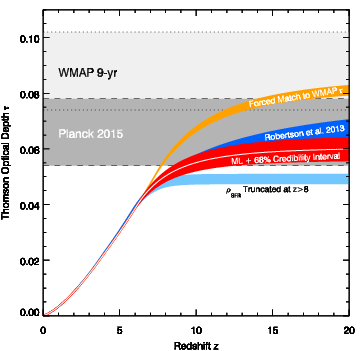
\includegraphics[width=.95\linewidth]{img/01/epaisseur_optique_thomson.png} 
        \caption{%https://inspirehep.net/record/1343310/plots
		Epaisseur optique Thomson
        Image Robertson et al.}
 		\label{fig:epaisseur_optique_thomson}
\end{figure}



polarisation du CMB

ligne 21 cm

fonction de luminosité UV



\section{Théorie -> La reionization}

réionisation et non rayonnisation!

Qu'est ce que c'est?

fin des âges sombres
apparition des première sources de rayonnement
Pourquoi étudier la réionisation

Dernier processus impactant l'ensemble de l'univers.
Importance pour le "missing satellite problem"

\subsection{Sphère de Stromgren}


\subsection{les principales question en suspend de l'étude de la réionisation}

quand est ce arrivé?
quelles sont les sources? -> débat galaxies vs quasars
\begin{figure}[bth]
        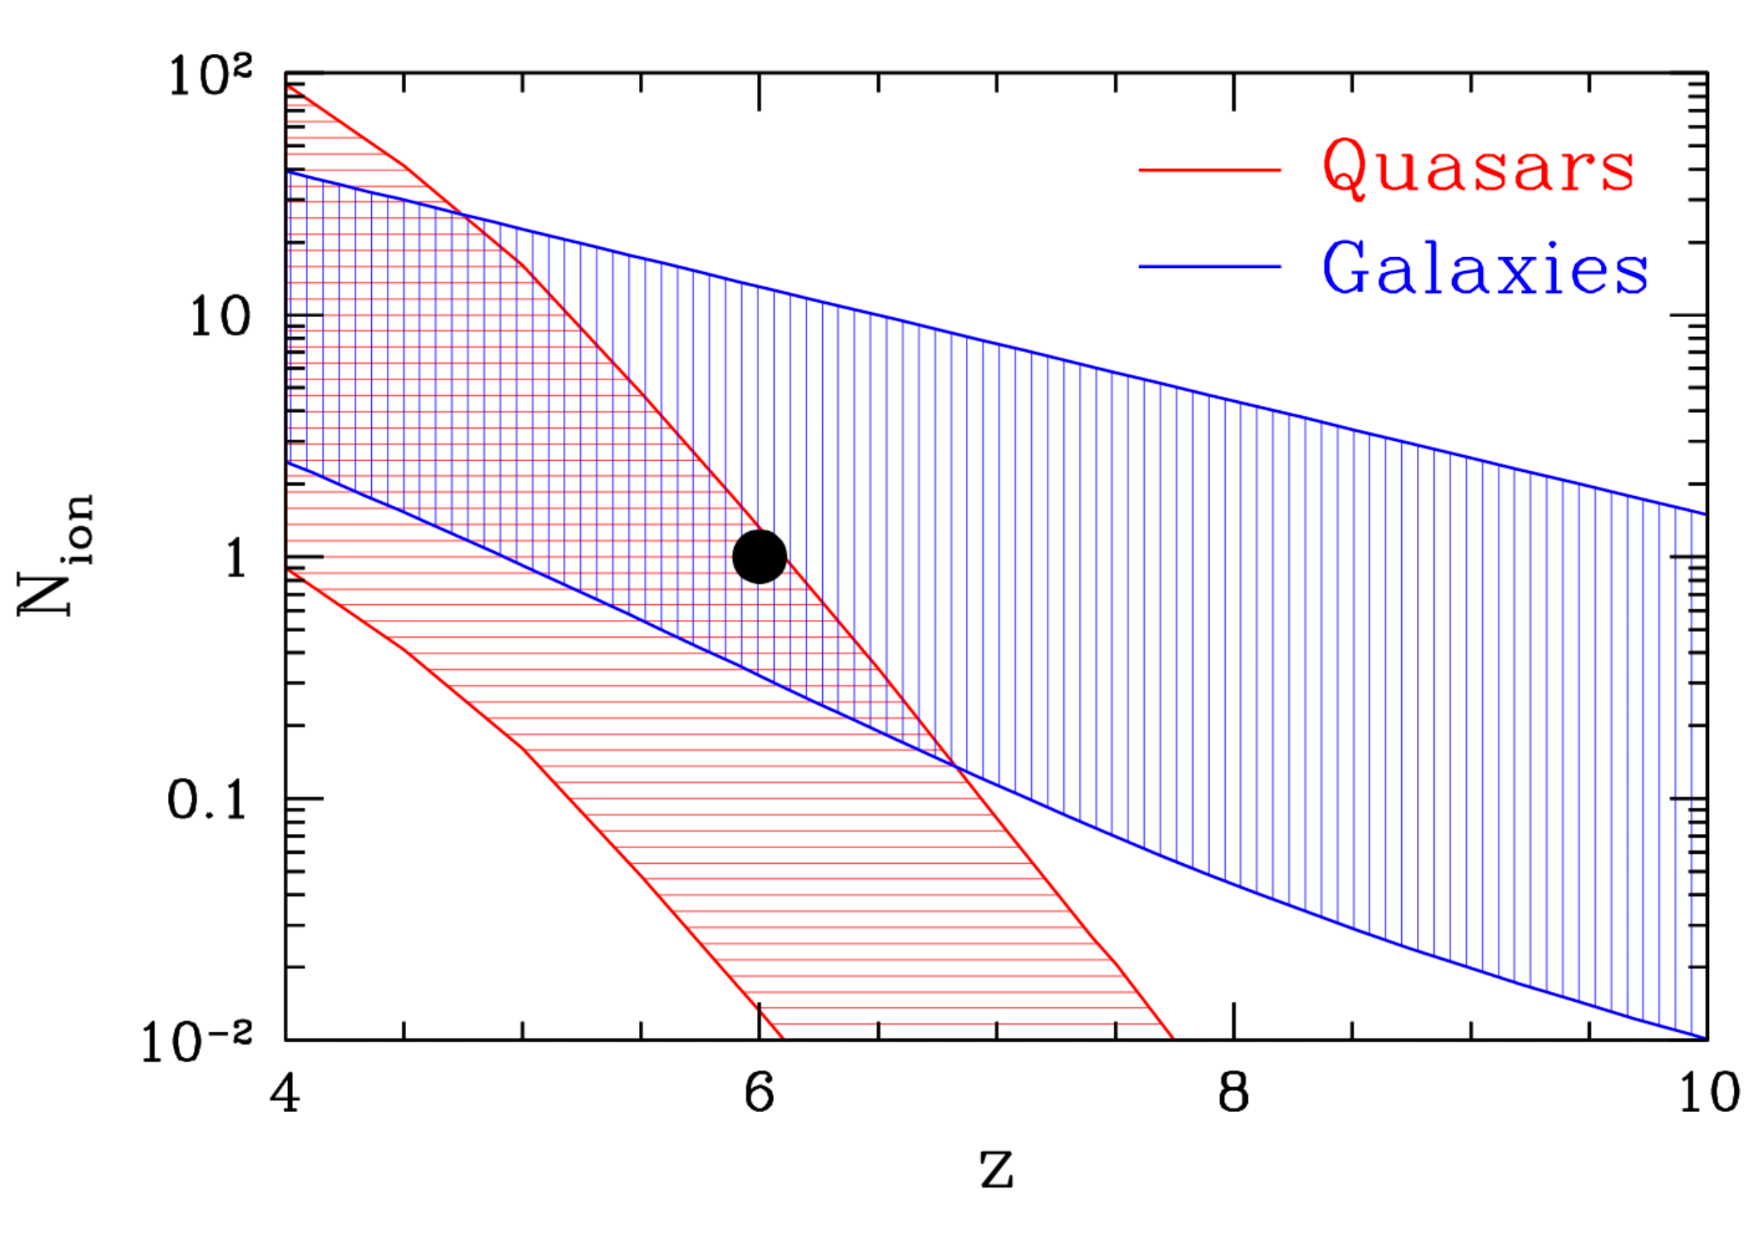
\includegraphics[width=.95\linewidth]{img/01/gal_AGN.pdf} 
        \caption{
        Budget de photons provenant des galaxies et des quasars qurant la reionization.
}
 		\label{fig:gal_AGN}
\end{figure}

outlier dans l'épaisseur optique des quasars
Le groupe local ?


